ie Langmuir-Isotherme ist das einfachste Sorptionsmodell, das physikalische Grundlagen besitzt. 
Es geht von folgenden Annahmen aus:

\begin{itemize}
\item Adsorption nur in einer einzelnen molekularen Schicht
\item alle Sorptionsplaetze sind gleichwertig
\item die Oberflaeche ist gleichfoermig 
\item keine Wechselwirkungen zwischen benachbarten Sorptionsplaetzen und den adsorbierten Teilchen
\end{itemize}

Die Langmuir-Isotherme kann eine maximale Beladung der Sorptionsoberflaechen abbilden und ist damit Ausgangsbasis für weitere Adsorptionsmodelle (Gleichung 1):

\begin{equation}
q=q_{max}*\frac{K*[Si]}{1+K*[Si]}
\end{equation}

\begin{description}
\item[ ] $q$ = adsorbierte Menge pro Gramm Gibbsit
\item[ ] $q_{max}$ = maximal adsorbierte Menge pro Gramm Gibbsit
\item[ ]$K$ = Langmuir Koeffizient	
\item[ ]$[Si]$ = Si concentration
\end{description}

\bigskip

Abbildung 1 zeigt die erreichte Beladung an Si pro Gramm Gibbsite gegen die initiale Si Konzentration der Experimente.
\begin{figure}[htbp]
\begin{center}
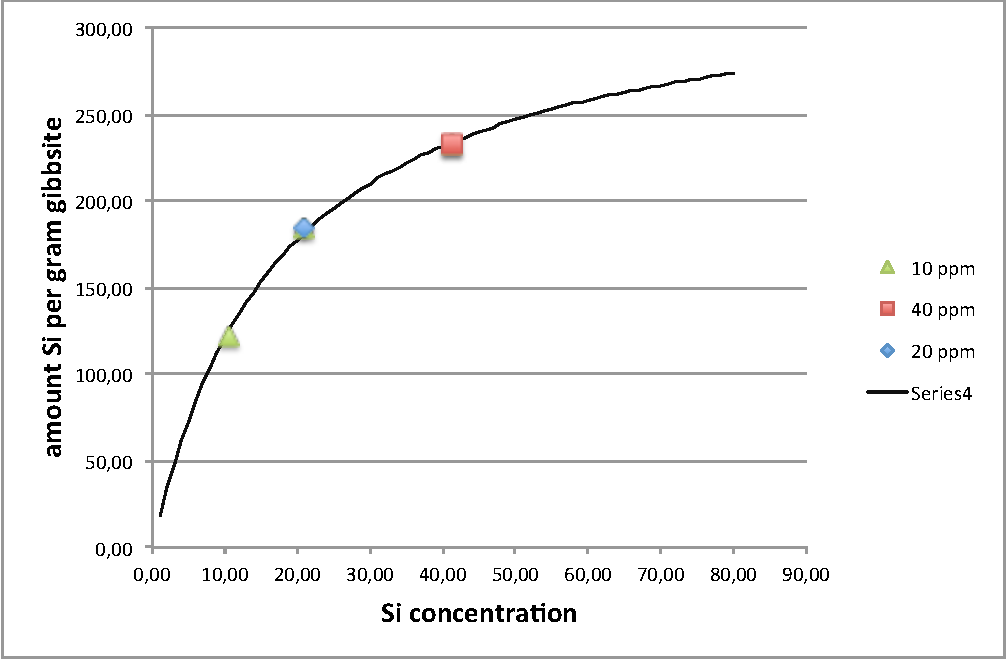
\includegraphics[width=11cm]{langmuir_fig.pdf}
\caption{Menge Si adsorbiert pro Gramm Gibbsit gegen die initiale Si Konzentration. Schware Kurve Adsorptionsisotherme nach Langmuir (Gleichung 1)}
\label{default}
\end{center}
\end{figure}


Lineraisieren nach Langmuir fuehrt zu Gleichung 2 und zur Abbildung 2:

\begin{equation}
\frac{[Si]}{q}=\frac{[Si]}{q_{max}}+\frac{1}{K*q{max}}
\end{equation}

\begin{figure}[htbp]
\begin{center}
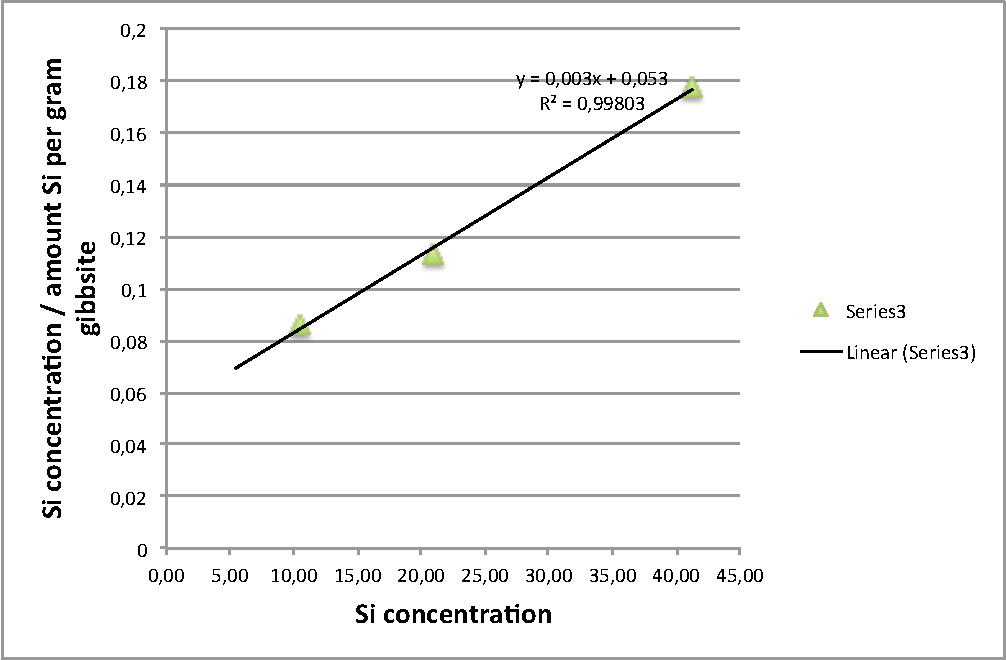
\includegraphics[width=11cm]{langmuir_fig_lin.pdf}
\caption{Si Konzentration geteilt durch die Menge Si adsorbiert pro Gramm Gibbsit ([Si]/q) gegen die Si Konzentration aufgetragen. Aus der Steigung kann man die maximale Beladung mit Si pro Gramm Gibbsite berechnen. }
\label{default}
\end{center}
\end{figure}

Aus der linearen Darstellung kann man aus der Steigung  eine maximale Beladung $q_{max}$ berechnen.
Dies ist hier $\sim$ 300$\mu$g Si pro Gramm Gibbsit ($1.2*10^{-5}$ mol Si pro Gramm Gibbsit)
Die maximal adsorbierte Menge in dieser Versuchsreihe waren  $\sim$ 230$\mu$g Si pro Gramm Gibbsite bei initial 40 ppm Si.

